\chapter{Zanka \texttt{for}}

\section{Sprehajanje čez sezname z zanko \texttt{for}}
Kot smo videli na koncu prejšnjega poglavja, se lahko čez seznam (ali niz) sprehodimo z uporabo zanke \texttt{while}, pri čemer sprehod vršimo preko indeksov seznama, preko katerih lahko posredno pridemo tudi do vrednosti elementov seznama (ali niza). Veliko bolj elegantno pa se čez seznam (ali pač niz) sprehodimo z uporabo zanke \texttt{for}:
\begin{lstlisting}[language=Python]
for element in seznam:
    # telo zanke
    # spremenljivka element vsebuje trenuten element
    ...
# nadaljevanje programa
...
\end{lstlisting}
Potek izvedbe osnovne oblike zanke \texttt{for} ponazarja slika \ref{img:for1}
\begin{figure}
    \centering
    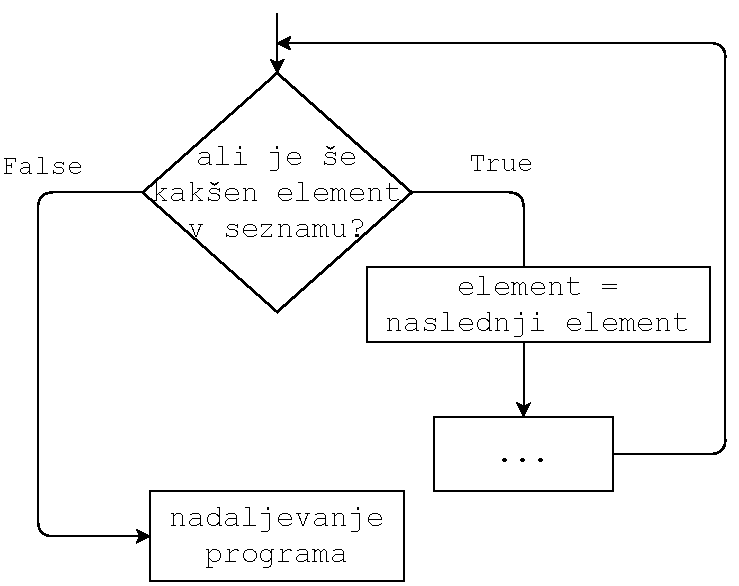
\includegraphics[width=0.5\linewidth]{img/for1.pdf}
    \caption{Potek izvedbe osnovne oblike zanke \texttt{for}.}
    \label{img:for1}
\end{figure}
Izvajanje zanke torej ponavljamo vse dokler je v seznamu (ali nizu) še kakšen element, pri čemer se spremenljivka \texttt{element} pomika od začetka proti koncu seznama (ali niza). Če bi npr. želeli izpisati vse elemente v seznamu, pri čemer bi vsak element izpisali v svoji vrstici, bi to lahko naredili takole:
\begin{lstlisting}[language=Python]
>>> seznam = [1,2,3]
>>> for element in seznam:
	print(element)
1
2
3
\end{lstlisting}
Na podoben način bi se lahko sprehodili tudi čez niz:
\begin{lstlisting}[language=Python]
>>> niz = "ABC"
>>> for znak in seznam:
	print(znak)
A
B
C
\end{lstlisting}
V tem primeru se zanka \texttt{for} torej sprehaja čez znake niza.

Povadimo sprehajanje še na zgledu.
\begin{zgled}
Napiši program, ki od uporabnika preko funkcije \texttt{eval} prebere seznam in izpiše najmanjši element seznama (brez uporabe funkcije \texttt{min}). 
\end{zgled}
\begin{resitev}
Najmanjši element bomo našli tako, da se bomo z zanko \texttt{for} sprehodili čez seznam in si zapomnili element, ki je pač najmanjši. Kako pa vemo, da je nek element najmanjši, če ostalih še nismo pregledali? Težko. Vemo pa, če je nek element manjši od vseh elementov, ki smo jih pregledali preden smo do njega prišli. Nalogo bomo torej rešili tako, da bomo začeli s predpostavko, da je najmanjši prvi element v seznamu. Potem bomo naredili sprehod čez celoten seznam. Če bomo našli kakšen element, ki je manjši od trenutno najmanjšega, bomo trenutno najmanjši element postavili na tega, ki je očitno manjši. To bomo nadaljevali, dokler ne pridemo do konca seznama.
\begin{lstlisting}[language=Python,numbers=left]
seznam = eval(input("Vnesi seznam: "))

najmanjsi = seznam[0] # trenutno najmanjsi

for element in seznam: # sprehod cez elemente
    if element < najmanjsi: # nasli manjsega?
        najmanjsi = element # popravimo vrednost

print(najmanjsi)
\end{lstlisting}
Program sicer deluje pravilno, ampak bi ga lahko še nekoliko optimizirali. Trenutno namreč ničti element v seznamu pregledamo dvakrat. Sprehoda z zanko \texttt{for} nam torej ne bi bilo potrebno delati čez cel seznam, ampak bi ga lahko naredili čez rezino seznama, ki se začne na indeksu 1. Torej bi zanko \texttt{for} lahko delali čez rezino \texttt{seznam[1:]}.
\end{resitev}

\section{Sprehajanje s funkcijo \texttt{range} in sprehajanje čez indekse}

Z zanko \texttt{for} se lahko sprehajamo tudi čez sezname, ki jih generira funkcija \texttt{range}. Na tak način se lahko sprehajamo čez vrednosti elementov v določenem razponu. Vsa števila od 0 do vključno števila, ki ga je vnesel uporabnik, bi torej lahko izpisali takole:
\begin{lstlisting}[language=Python]
n = int(input("Vnesi stevilo: "))
for i in range(n+1):
    print(i)
\end{lstlisting}

Zanko \texttt{for} bi lahko na podoben način uporabili za sprehajanje po indeksih seznama. Vrednosti v seznamu na posameznih indeksih bi lahko izpisali takole:
\begin{lstlisting}[language=Python]
for i in range(len(seznam)):
    print(i, seznam[i])
\end{lstlisting}
Tokrat funkciji \texttt{range} kot argument \texttt{stop} podamo dolžino seznama, kar pomeni, da bo funkcija zgenerirala razpon elementov v intervalu od 0 do \texttt{len(seznam)-1}, kar je ravno razpon indeksov seznama. Zato torej argument \texttt{stop} v interval ni vključen in zato funkcija \texttt{range} (tudi) deluje kakor deluje.

\section{Sprehajanje čez elemente ali čez indekse?}
Zgornji program bo poleg indeksa izpisal še vrednost elementa, ki se nahaja na posameznem indeksu. Ali bi lahko do indeksa elementov prišli tudi v primeru, ko se sprehajamo neposredno po elementih seznama? Težko. Zato v primeru, ko informacijo in indeksu potrebujemo, uporabljamo zanko čez indekse in ne čez elemente.  

Poglejmo si spodnji primer, kjer rešitev zahteva izvedbo sprehoda čez indekse seznama.
\begin{zgled}
Napiši program, ki od uporabnika preko funkcije \texttt{eval} prebere seznam in izpiše najmanjši element seznama ter njegov indeks. 
\end{zgled}
\begin{resitev}
Najmanjši element bomo našli na podoben način kot prej, le da si moramo tokrat zapomniti tudi njegov indeks. Ker preko direktnega sprehoda čez elemente seznama informacije o indeksih elementov nimamo, se bomo morali sprehoditi čez indekse seznama.
\begin{lstlisting}[language=Python,numbers=left]
seznam = eval(input("Vnesi seznam: "))

najmanjsi = seznam[0] # trenutno najmanjsi element
najmanjsi_i = 0 # zapomnimo si tudi njegov indeks

for i in range(len(seznam)): # sprehod cez indekse
    element = seznam[i] # preko indeksa do elementa
    if element < najmanjsi: # nasli manjsega?
        najmanjsi = element # popravimo vrednost
        najmanjsi_i = i # popravimo indeks

print(najmanjsi)
print(najmanjsi_i)
\end{lstlisting}
Spet bi lahko pri sprehodu prvi element seznama izpustili, tako da bi se sprehajali čez razpon \texttt{range(1, len(seznam))}.
\end{resitev}

Zgornja rešitev ima manjšo pomanjkljivost, in sicer ne upošteva, da se lahko enako majhen element v seznamu pojavi večkrat. V tem primeru vrne zgolj indeks njegove prve pojavitve. Naprednejšo rešitev prikazuje spodnji zgled.

\begin{zgled}
Napiši program, ki od uporabnika preko funkcije \texttt{eval} prebere seznam in izpiše najmanjši element seznama ter vse indekse njegove pojavitve. 
\end{zgled}
\begin{resitev}
Rešitev bo podobna kot prej, le da si bomo indekse pojavitve najmanjšega elementa zabeležili kar v seznam. V primeru, da bomo našli manjši element od trenutnega, bomo naredili nov seznam, ki bo vseboval samo en indeks (trenutni indeks). V primeru, da bomo našli element, ki bo enak trenutno najmanjšemu, bomo v seznam indeksov dodali trenutni indeks. V zgornjih dveh rešitvah smo na koncu dodali boljšo rešitev, ki pri sprehodu izpusti ničti element seznama, saj smo tega upoštevali že pred zanko. Tokrat bo program brez te "optimizacije"  deloval narobe. V primeru, da bo najmanjši element na ničtem mestu, bo njegov indeks v seznamu najmanjših indeksov namreč nastopač dvakrat.
\begin{lstlisting}[language=Python,numbers=left]
seznam = eval(input("Vnesi seznam: "))

najmanjsi = seznam[0] # trenutno najmanjsi element
najmanjsi_i = [0] # v seznam shranimo njegov indeks

for i in range(len(seznam)): # sprehod cez indekse
    element = seznam[i] # preko indeksa do elementa
    if element < najmanjsi: # nasli manjsega?
        najmanjsi = element # popravimo vrednost
        najmanjsi_i = [i] # resetiramo seznam indeksov
    elif element == najmanjsi: # nasli enako majhnega
        najmanjsi_i.append(i) # dodamo indeks

print(najmanjsi)
print(najmanjsi_i)
\end{lstlisting}
\end{resitev}

\section{Spreminjanje elementov seznama z zanko \texttt{for}}
Kaj pa v primeru da želimo seznam v zanki spremeniti, npr. da želimo seznam spremeniti, tako da bo vse negativne vrednosti spremenil v pozitivne (izračunati želimo absolutne vrednosti elementov seznama in seznam skladno s tem posodobiti). Poskusimo z običajnim sprehodom čez elemente seznama.
\begin{lstlisting}[language=Python]
>>> seznam = [-1, 10, -5, 15, 0, -3]
>>> for element in seznam:
	element = abs(element)
	print(element)
1
10
5
15
0
3
>>> print(seznam)
[-1, 10, -5, 15, 0, -3]
\end{lstlisting}
Elemente smo torej uspešno postavili na njihove absolutne vrednosti, na kar nakazujejo izpisi, ki smo jih izvedli v telesu zanke. Kot pa vidimo iz izpisa, ki je sledil zanki, se seznam ni spremenil, saj še vedno vsebuje negativne elemente. Spreminjali smo torej vrednosti elementov, ne pa samega seznama. Če bi želeli spreminjati seznam, bi to lahko naredili preko indeksiranja:
\begin{lstlisting}[language=Python]
>>> seznam = [-1, 10, -5, 15, 0, -3]
>>> for i in range(len(seznam)):
	seznam[i] = abs(seznam[i])
	print(seznam[i])
1
10
5
15
0
3
>>> print(seznam)
[1, 10, 5, 15, 0, 3]
\end{lstlisting}
Zdaj se je seznam seveda spremenil, saj smo absolutne vrednosti prirejali vrednostim, ki stojijo za posameznim indeksom.

\section{Zanka \texttt{for} ali zanka \texttt{while}?}
Vidimo, da so naši programi z uporabo zanke \texttt{for} v določenih veliko krajši in lepši kot v primeru uporabe zanke \texttt{while}. Zakaj bi torej sploh uporabljali zanko \texttt{while}? Izkaže se, da je zanka \texttt{while} bolj splošna kot zanka \texttt{for} in da lahko z njo rešimo določene probleme, ki jih z zanko \texttt{for} ne moremo. Kako bi npr. z zanko \texttt{for} od sodnika smučarskih skokov brali dolžine skokov, dokler sodnik ne vnese števila 0? Koliko ponovitev bi morali narediti? Kako bi z zanko \texttt{for} odštevali manjše število od večjega, dokler števili ne bi postali enaki? Odgovor je težko.

Vprašajmo se, kaj je skupnega primerom, kjer zanka \texttt{for} odpove. V obeh zgornjih primerih je število ponovitev, ki jih bo morala zanka narediti, vnaprej težko predvidljivo. V splošnem velja, da zanko \texttt{while} uporabljamo kadar število ponovitev zanke težko podamo vnaprej, lahko pa oblikujemo pogoj, ki bo določil, do kdaj naj se zanka izvaja. V primeru, da je število ponovitev predvidljivo (npr. podan je razpon štetja ali pa seznam s fiksno dolžino, čez katerega se sprehajao) pa je kot nalašč zanka \texttt{for}.

\section{Stavek \texttt{break}}

V kombinaciji z zanko \texttt{for} lahko prav tako kot pri zanki \texttt{while} uporabljamo stavek \texttt{break}. Ta izvajanje zanke prekine, kljub temu, da ta še ni prišla do konca seznama (ali česa drugega). Primer uporava stavka \texttt{break} znotraj zanke \texttt{while} ponazarja spodnja koda:
\begin{lstlisting}[language=Python]
for element in seznam:
    # telo zanke
    ...
    if dodaten_pogoj: 
        break # prekine izvajanje zanke
# nadaljevanje programa
...
\end{lstlisting}
Potek izvedbe kode iz primera prikazuje slika \ref{img:for2}.
\begin{figure}
    \centering
    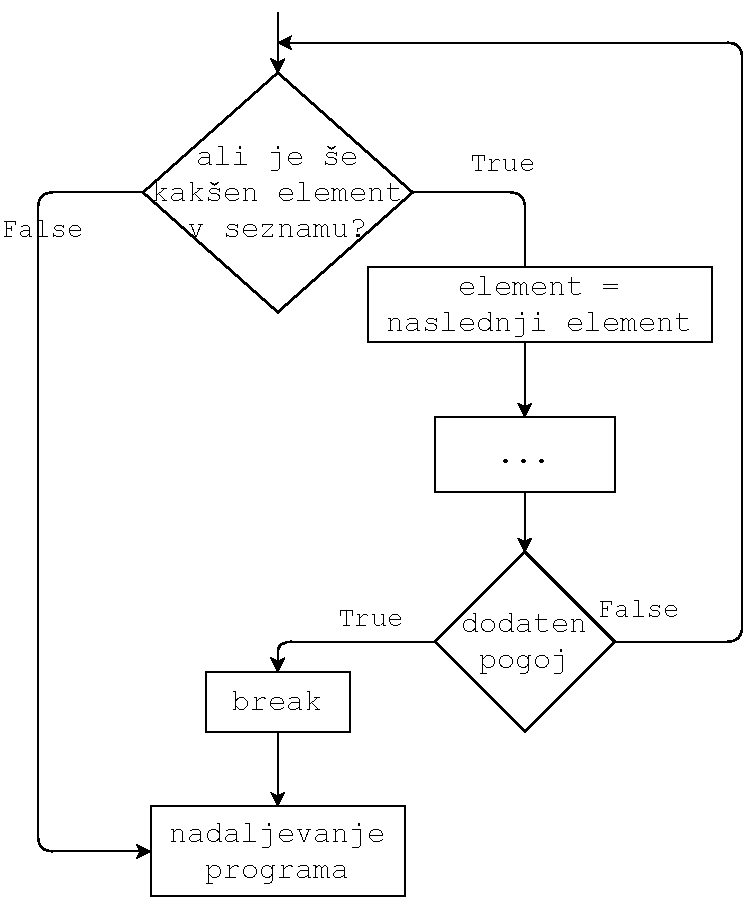
\includegraphics[width=0.5\linewidth]{img/for2.pdf}
    \caption{Potek izvedbe zanke \texttt{for} v kombinaciji s stavkom \texttt{break}.}
    \label{img:for2}
\end{figure}


\section{Veja \texttt{else}}

Podobno kot lahko vejo \texttt{else} kombiniramo z zanko \texttt{while}, jo lahko kombiniramo tudi z zanko \texttt{for}:
\begin{lstlisting}[language=Python]
for element in seznam:
    # telo zanke
    ...
    if dodaten_pogoj:
        break # prekini izvajanje zanke
else: # samo v primeru, ko zanka ni bila prekinjena z break
    # konec seznama
    ...
# nadaljevanje programa
...
\end{lstlisting}

Veja \texttt{else} se bo kot pri zanki \texttt{while} izvedla samo v primeru, ko zanka ni bila prekinjena s stavkom \texttt{break}. Demonstrirajmo uporabo koncepta na enakem zgledu.

\begin{zgled}
Napiši program, ki od uporabnika prebere dve celi števili in izpiše, če sta števili tuji. Števili sta tuji, če nimata nobenega skupnega delitelja, ki je večji od 1.
\end{zgled}
\begin{resitev}
Program bo strukturiran zelo podoben kot v primeru zanke \texttt{while}, le da bomo tokrat razpon števil, čez katera se sprehaja kandidat ustvarili z uporabo funkcije \texttt{range}. 

\begin{lstlisting}[language=Python,numbers=left]
st1 = int(input("Vnesi prvo stevilo: "))
st2 = int(input("Vnesi drugo stevilo: "))

# sprehod od 2 do manjsega od obeh stevil
# desni del intervala naj bo vkljucen, zato pristejemo 1
for delitelj in range(2,min(st1, st2)+1):
    # ali delitelj deli obe stevili?
    if st1 % delitelj == 0 and st2 % delitelj == 0:
        print("Stevili nista tuji")
        break # lahko prenehamo z iskanjem
else: # ali se je zanka odvrtela do konca
    # zanke nismo prekinili s stavkom break
    print("Stevili sta tuji")
\end{lstlisting}
\end{resitev}


\section{Gnezdenje zank}

Podobno kot smo gnezdili stavke \texttt{if} lahko gnezidmo tudi zanke. To pomeni, da bomo zanko izvajali znotraj druge zanke. Primer gnezdenja zanke \texttt{for} prikazuje spodnji izsek kode:
\begin{lstlisting}[language=Python]
>>> for i in range(5):
        for j in range(5):
            print(i,j)
0 0
0 1
0 2
0 3
0 4
1 0
1 1
...
3 3
3 4
4 0
4 1
4 2
4 3
4 4
\end{lstlisting}
Notraja zanka \texttt{for} torej za vsako iteracijo zunanje zanke izvede enako število ponovitev.

Potrenirajmo na zgledu.

\begin{zgled}
Napiši program, ki od uporabnika prebere celo število in izpiše poštevanko števil od 1 do vključno podanega števila.
\end{zgled}
\begin{resitev}
Števila od 1 do podanega števila \texttt{n} bomo najprej množili z 1, potem z 2, potem s 3 in tako naprej, dokler ne pridemo do števila \texttt{n}. To lahko enostavno rešimo z uporaba ugnezdene zanke.
\begin{lstlisting}[language=Python]
n = int(input("Vnesi stevilo: "))

for i in range(1, n+1): # zunanja zanka
    for j in range(1, n+1): # notranja zanka
        print(i*j) # izpis produkta
    print() #nova vrstica
\end{lstlisting}
V primeru, da uporabnik vpiše število 3, bo izpis sledeč:
\begin{lstlisting}[language=Python]
1
2
3

2
4
6

3
6
9
\end{lstlisting}
\end{resitev}

V zgornjih primerih je bila notranja zanka neodvisna od tega, kako daleč se je že odvila notranja zanka. Ponavadi pa temu ni tako. Primer ugnezdene zanke, pri kateri je razpon notranje zanke odvisen od števila izvedenih iteracij zunanje zanke, prikazuje spodnji izsek kode:
\begin{lstlisting}[language=Python]
>>> for i in range(5):
        for j in range(i,5):
            print(i,j)
0 0
0 1
0 2
0 3
0 4
1 1
1 2
1 3
1 4
2 2
2 3
2 4
3 3
3 4
4 4
\end{lstlisting}
V prvi iteraciji zunanje zanke, se torej notranja zanka izvede petkrat, v drugi štirikrat, v tretji trikrat, v četrti dvakrat, v peti pa zgolj enkrat. Kasnejša kot je iteracija zunanje zanke, manjše je število ponovitev ugnezdene zanke. 

Povadimo tako gnezdenje še na primeru s tujimi števili.
\begin{zgled}
Napiši program, ki od uporabnika prebere celo število in izpiše vsa števila, ki so podanemu številu tuja in so od njega manjša. 
\end{zgled}
\begin{resitev}
Kandidati, ki jih moramo torej obravnavati, se gibljejo v razponu od števila 1 (ki je vsem številom tuje število) do števila \texttt{n-1}, pri čemer je \texttt{n} število, ki ga je vnesel uporabnik. Kako za posameznega kandidata preverimo, če je tuj številu \texttt{n}? Podobno kot prej -- tako da se sprehodimo od števila 2, do manjšega od obeh števil. Če smo našli kakšnega delitelja, si števili očitno nista tuji.
\begin{lstlisting}[language=Python,numbers=left]
n = int(input("Vnesi stevilo: "))

for kandidat in range(1, n): # razpon cez kandidate
    # kandidat ne sme imeti nobenega skupnega delitelja
    # ugnezdimo kodo iz prejsnjih zgledov
    st1 = n
    st2 = kandidat
    
    # sprehod od 2 do manjsega od obeh stevil
    # desni del intervala naj bo vkljucen, zato pristejemo 1
    for delitelj in range(2,min(st1, st2)+1):
        # ali delitelj deli obe stevili?
        if st1 % delitelj == 0 and st2 % delitelj == 0:
            break # lahko prekinemo ugnezdeno zanko
    else: # ali se je ugnezdena zanka odvrtela do konca
        # ugnezdene zanke nismo prekinili s stavkom break
        print(kandidat)
\end{lstlisting}
\end{resitev}
Ugnezdena zanka je v tem primeru odvisna od tega kako daleč je naš program prišel z zunanjo zanko. Mimogrede, na podoben način bi lahko gnezdili tudi zanko \texttt{while}. 


\section{Izbirni argumenti funkcij in izbirni argumenti funkcije \texttt{print}}

Tole sicer ni neposredno povezano z zanko \texttt{for}, bo pa služilo kot osnova za dopolnitev zgleda s poštevanko. 

Povedali smo že, da funkcije sprejemajo argumente, ki jih ob klicu pač podamo. V določenih primerih pa imajo funkcije tudi t.i. \emph{izbirne} ali \emph{opcijske} argumente, za katere velja da imajo \emph{privzeto} vrednost nastavljeno. V primeru, da vrednosti teh argumentov eksplicitno ne podamo, bodo ti nastavljeni na njihove privzete vrednosti. V primeru, da vrednosti tem argumentom podamo, bomo s tem \emph{povozili} privzete vrednosti in uporabljene bodo podane vrednosti.

Poglejmo si dva izbirna argumenta funkcije \texttt{print} in primer njune uporabe. Do dokumentacije funkcije \texttt{print} lahko pridemo preko funkcije \texttt{help}:
\begin{lstlisting}[language=Python]
>>> help(print)
Help on built-in function print in module builtins:

print(...)
    print(value, ..., sep=' ', end='\n', file=sys.stdout, 
    flush=False)
    
    Prints the values to a stream, or to sys.stdout by default.
    Optional keyword arguments:
    file:  a file-like object (stream); defaults to the current 
    sys.stdout.
    sep:   string inserted between values, default a space.
    end:   string appended after the last value, default a newline.
    flush: whether to forcibly flush the stream.
\end{lstlisting}
Zaenkrat nas bosta zanimala predvsem argumenta \texttt{sep} in \texttt{end}. Funkcija \texttt{print} deluje tako, da sprejme poljubno število številk, nizov in še česa drugega, to med seboj združi in izpiše na zaslon. Pri tem argument \texttt{sep} določa s čim naj podane številke, nize in še kaj drugega med seboj združi. Privzeto je ta argument postavljen na vrednost \texttt{' '}, kar vidimo iz zgleda klica funkcije (\texttt{sep=' '}). To pomeni, da bo izpis narejen tako, da bodo med podanimi argumenti za izpis vstavljeni presledki. Povadimo:
\begin{lstlisting}[language=Python]
>>> print(1,2,3) # privzeta vrednost argumenta
1 2 3
>>> print(1,2,3, sep='') # brez presledka
123
>>>print(1,2,3, sep='+++') # poljuben niz kot locilo
1+++2+++3
\end{lstlisting}
Izbirni argument \texttt{end} podaja niz, ki naj se vstavi na koncu izpisa. Privzeto je argument \texttt{end} nastavljen na znak \texttt{'$\backslash$n'} (\texttt{end='$\backslash$n'}), ki podaja znaka za novo vrstico \angl{line feed}. Tudi tega lahko postavimo na kakšno drugo vrednost. 

Povadimo nastavljanje opcijskih argumentov na zgledu v kombinaciji z ugnezdeno zanko \texttt{for}.

\begin{zgled}
Napiši program, ki od uporabnika prebere celo število in izpiše poštevanko števil od 1 do vključno podanega števila. Pri tem naj bo poštevanka s posameznim številom podana v svoji vrstici, števila pa naj bodo ločena s presledki.
\end{zgled}
\begin{resitev}
Rešitev bo podobna kot prej, le da se tokrat ne bomo pomikali v novo vrstico po vsakem izpisu. To lahko naredimo tako, da opcijski argument  \texttt{end} nastavimo na znak \texttt{' '}.

\begin{lstlisting}[language=Python]
n = int(input("Vnesi stevilo: "))

for i in range(1, n+1): # zunanja zanka
    for j in range(1, n+1): # notranja zanka
        print(i*j, end = ' ') # izpis produkta brez nove vrstice
    print() #nova vrstica
\end{lstlisting}
V primeru, da uporabnik vpiše število 3, bo tokrat izpis sledeč:
\begin{lstlisting}[language=Python]
1 2 3
2 4 6
3 6 9
\end{lstlisting}
\end{resitev}
